\documentclass[12pt]{article}
%%%%%%%%%%%%%%%%%%%%%%%%%%%%%%%%%%%%%%%%%%%%%%%%%%%%%%%%%%%%%
% Meta informations:
\newcommand{\trauthor}{Michael Hüppe}
\newcommand{\trtype}{Paper} %{Expos\'{e}} %{Review}
\newcommand{\trtitle}{Diffusion Model for Generating new Pokémon}
\newcommand{\trdate}{08.12.2023}

%%%%%%%%%%%%%%%%%%%%%%%%%%%%%%%%%%%%%%%%%%%%%%%%%%%%%%%%%%%%%
% Languages:

% Falls die Ausarbeitung in Deutsch erfolgt:
% \usepackage[german]{babel}
% \usepackage[T1]{fontenc}
% \usepackage[latin1]{inputenc}
% \usepackage[latin9]{inputenc}	 				
% \selectlanguage{german}

% If the thesis is written in English:
\usepackage[english]{babel} 
\usepackage{acronym}

% Define abbreviations using \acrodef{<label>}{<abbreviation>}
\acrodef{HTML}{Hypertext Markup Language}
\acrodef{GAN}{Generative Adversarial Network}
\acrodef{DCGAN}{Deep Convolutional Generative Adversarial Network}
\acrodef{DDPM}{Denoising Diffusion Probabilistic Models}
\acrodef{MSE}{Mean-square Error}
\usepackage{enumitem}				
\selectlanguage{english}

%%%%%%%%%%%%%%%%%%%%%%%%%%%%%%%%%%%%%%%%%%%%%%%%%%%%%%%%%%%%%
% Bind packages:
\usepackage{acronym}                    % Acronyms
\usepackage{algorithmic}								% Algorithms and Pseudocode
\usepackage{algorithm}									% Algorithms and Pseudocode
\usepackage{amsfonts}                   % AMS Math Packet (Fonts)
\usepackage{amsmath}                    % AMS Math Packet
\usepackage{amssymb}                    % Additional mathematical symbols
\usepackage{hyperref}             % Additional mathematical symbols
\usepackage{amsthm}
\usepackage{booktabs}                   % Nicer tables
%\usepackage[font=small,labelfont=bf]{caption} % Numbered captions for figures
\usepackage{color}                      % Enables defining of colors via \definecolor
\definecolor{uhhRed}{RGB}{254,0,0}		  % Official Uni Hamburg Red
\definecolor{uhhGrey}{RGB}{122,122,120} % Official Uni Hamburg Grey
\usepackage{fancybox}                   % Gleichungen einrahmen
\usepackage{fancyhdr}										% Packet for nicer headers
%\usepackage{fancyheadings}             % Nicer numbering of headlines

%\usepackage[outer=3.35cm]{geometry} 	  % Type area (size, margins...) !!!Release version
%\usepackage[outer=2.5cm]{geometry} 		% Type area (size, margins...) !!!Print version
%\usepackage{geometry} 									% Type area (size, margins...) !!!Proofread version
\usepackage[outer=3.15cm]{geometry} 	  % Type area (size, margins...) !!!Draft version
\geometry{a4paper,body={5.8in,9in}}

\usepackage{graphicx}                   % Inclusion of graphics
%\usepackage{latexsym}                  % Special symbols
\usepackage{longtable}									% Allow tables over several parges
\usepackage{listings}                   % Nicer source code listings
\usepackage{multicol}										% Content of a table over several columns
\usepackage{multirow}										% Content of a table over several rows
\usepackage{rotating}										% Alows to rotate text and objects
\usepackage[hang]{subfigure}            % Allows to use multiple (partial) figures in a fig
%\usepackage[font=footnotesize,labelfont=rm]{subfig}	% Pictures in a floating environment
\usepackage{tabularx}										% Tables with fixed width but variable rows
\usepackage{url,xspace,boxedminipage}   % Accurate display of URLs

%%%%%%%%%%%%%%%%%%%%%%%%%%%%%%%%%%%%%%%%%%%%%%%%%%%%%%%%%%%%%
% Configurationen:

\hyphenation{whe-ther} 									% Manually use: "\-" in a word: Staats\-ver\-trag

%\lstloadlanguages{C}                   % Set the default language for listings
\DeclareGraphicsExtensions{.pdf,.svg,.jpg,.png,.eps} % first try pdf, then eps, png and jpg
\graphicspath{{./src/}} 								% Path to a folder where all pictures are located
\pagestyle{fancy} 											% Use nicer header and footer

% Redefine the environments for floating objects:
\setcounter{topnumber}{3}
\setcounter{bottomnumber}{2}
\setcounter{totalnumber}{4}
\renewcommand{\topfraction}{0.9} 			  %Standard: 0.7
\renewcommand{\bottomfraction}{0.5}		  %Standard: 0.3
\renewcommand{\textfraction}{0.1}		  	%Standard: 0.2
\renewcommand{\floatpagefraction}{0.8} 	%Standard: 0.5

% Tables with a nicer padding:
\renewcommand{\arraystretch}{1.2}

%%%%%%%%%%%%%%%%%%%%%%%%%%%%
% Additional 'theorem' and 'definition' blocks:
\theoremstyle{plain}
\newtheorem{theorem}{Theorem}[section]
%\newtheorem{theorem}{Satz}[section]		% Wenn in Deutsch geschrieben wird.
\newtheorem{axiom}{Axiom}[section] 	
%\newtheorem{axiom}{Fakt}[chapter]			% Wenn in Deutsch geschrieben wird.
%Usage:%\begin{axiom}[optional description]%Main part%\end{fakt}

\theoremstyle{definition}
\newtheorem{definition}{Definition}[section]

%Additional types of axioms:
\newtheorem{lemma}[axiom]{Lemma}
\newtheorem{observation}[axiom]{Observation}

%Additional types of definitions:
\theoremstyle{remark}
%\newtheorem{remark}[definition]{Bemerkung} % Wenn in Deutsch geschrieben wird.
\newtheorem{remark}[definition]{Remark} 

%%%%%%%%%%%%%%%%%%%%%%%%%%%%
% Provides TODOs within the margin:
\newcommand{\TODO}[1]{\marginpar{\emph{\small{{\bf TODO: } #1}}}}

%%%%%%%%%%%%%%%%%%%%%%%%%%%%
% Abbreviations and mathematical symbols
\newcommand{\modd}{\text{ mod }}
\newcommand{\RS}{\mathbb{R}}
\newcommand{\NS}{\mathbb{N}}
\newcommand{\ZS}{\mathbb{Z}}
\newcommand{\dnormal}{\mathit{N}}
\newcommand{\duniform}{\mathit{U}}

\newcommand{\erdos}{Erd\H{o}s}
\newcommand{\renyi}{-R\'{e}nyi}
\usepackage[backend=biber,style=apa, natbib=true]{biblatex}
\DefineBibliographyStrings{english}{andothers = {\emph{et al}\adddot}}
\addbibresource{main.bib} % The filename of the bibliography
%%%%%%%%%%%%%%%%%%%%%%%%%%%%%%%%%%%%%%%%%%%%%%%%%%%%%%%%%%%%%
% Document:
\begin{document}
\renewcommand{\headheight}{14.5pt}

\fancyhead{}
\fancyhead[CO]{\trtitle}

%%%%%%%%%%%%%%%%%%%%%%%%%%%%
% Cover Header:
\title{\trtitle\\[0.3cm]{\normalsize\trtype}}
\author{\trauthor}
\date{\trdate}
\maketitle

%%%%%%%%%%%%%%%%%%%%%%%%%%%%

\thispagestyle{empty}
\pagenumbering{arabic}
%
%% Abstrt gives a brief summary of the main points of a paper:
\begin{abstract}
Making its gaming debut in 1996 with "Pokémon Red and Green" and earning approximately 368 million from game sales alone, the Pokémon series stands as one of Nintendo's oldest and most well-known franchises. With a unique blend of character designs and turn-based role-playing, the game introduced an entire generation to a distinctive gaming style, earning its place as the seventh most successful game of all time. Consequently, the franchise's current cultural significance comes as no surprise.

The community's embrace of "Fakémons," or self-made Pokémon, has reached a point where these creations feature prominently in entire fan-made games. This widespread enthusiasm paved the way for the exploration of generating new Pokémon through the application of deep learning. In recent years the generation of images has become more popular with the easy access to generative networks such as \href{https://openai.com/blog/dall-e/}{DALL-E}, \href{https://github.com/NVlabs/stylegan2}{StyleGAN2} or \href{https://www.openai.com/research/gpt}{GPT-3}. Diffusion models describe one of the most popular architectures.	This paper outlines the methodology employed for scraping and standardizing the data, along with the construction of the network architecture.\\

\end{abstract}

% the actual content, usually separated over a number of sections
% each section is assigned a label, in order to be able to put a
% crossreference to it

\section{Introduction}
\label{sec:introduction}

\begin{itemize}
	\item provide overview of the importance and possible applications of the 3D object detection (possibly extending the ones names by )
	\item describe the motivation for using machine learning in 3D object detection
	\item motivate why we want to reproduce the findings from 
	\item outline the structure of the paper
\end{itemize}
%
%
\section{Related Work}
\label{sec:relwork}
Generating Pokémon using deep learning is not a novel idea. \cite{Kleiber2020} used a \ac{GAN} to create new Pokémon based on a dataset of ~800 data samples. The presented results seen in Figure \ref{fig:kleiberresults} can definitely be approved upon.\\
 

 \begin{figure}[h]
	\centering
	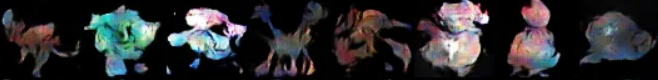
\includegraphics[width=1\linewidth]{src/Images/Kleiber_results}
	\caption[Results of \cite{Kleiber2020}]{Results of \cite{Kleiber2020}. The object somewhat resemble the colour scheme and form of a Pokémons. However, no image is recognizable as a complete design.}
	\label{fig:kleiberresults}
\end{figure}

Using the same dataset \cite{Chambel2022} trained a \ac{DCGAN} and achieved better results. The colour of the generated images is much closer to the often vibrant colour presented in the dataset. The results can be seen in Figure \ref{fig:chambelresults}.

\begin{figure}[h]
	\centering
	
\includegraphics[width=1\linewidth]{src/Images/Chambel_results}
	\caption[Results presented by \cite{Chambel2022}]{Results presented by \cite{Chambel2022}.}
	\label{fig:chambelresults}
\end{figure}


\section{Background}
\label{sec:background}
\cite{Ho2020} present a new generative deep neural network architecture called the \ac{DDPM}. 
%
\section{Data Acquisition and Preprocessing}
\label{sec:dataAca_and_preprocessing}
\subsection{Acquisition}
There is no official Pokémon dataset that provides the extensive sample size typically required for training generative deep learning models \citep{Yang2023}. Most of the available datasets offer only one image per Pokémon, resulting in approximately 1000 images in total. In comparison, the \href{https://www.cs.toronto.edu/~kriz/cifar.html}{cifar10} dataset consists of 60,000 samples. Moreover, each Pokémon has a unique and easily distinguishable design, making it challenging to identify similarities between them. To address this limitation, I opted to create my own Pokémon dataset using web scraping.

I used web scraping to extract data from the \href{https://pokemondb.net/}{Pokémon database}, which lists all Pokémon along with various design variations for each. The Python packages \href{https://www.crummy.com/software/BeautifulSoup/bs4/doc/}{BeautifulSoup} and \href{https://requests.readthedocs.io/en/latest/}{requests} packages provide functions to parse the website into \ac{HTML} and identify relevant tags. The \href{https://pokemondb.net/pokedex/national}{national Pokédex} which provides a list of all current Pokémon organized by Generation \footnote{In the context of Pokémon, a "generation" refers to a specific group or series of Pokémon games released by Nintendo and Game Freak. Each generation introduces a new set of Pokémon species, game mechanics, and often a new region to explore.} represents the start point of the acquisition pipeline.

We collected links for each entry, simplifying the retrieval of all accessible images through a systematic naming convention. The link structure is as follows: "pokemondb.net/identifier/Pokémon." Changing the identifier granted access to two distinct datasets. The "artwork" identifier encompassed both official and alternative artwork, while the "sprites" section stored all in-game renditions of the Pokémon. In total, we obtained 26,896 unique images (22,825 sprites and 4,071 artworks). The term "unique" requires caution, as we intentionally included both male and female versions (even if differing by minor details) and normal and shiny versions (same Pokémon but with different color coding). Additionally, the database provides GIFs depicting the idle animation of the Pokémon. Each frame of these animations were added to the dataset. The back view of Pokémon were ignored since the goal was to generate images from the front. 

The code for web scraping the images can be found \href{https://github.com/mhueppe/Diffusion_Models/tree/master/preprocessing}{here}. Figure \ref{fig:variouscharizard} shows an example of artworks and sprites for the Pokémon entry for \href{https://pokemondb.net/pokedex/charizard}{Charizard}.

\begin{figure}[h]
	\centering
	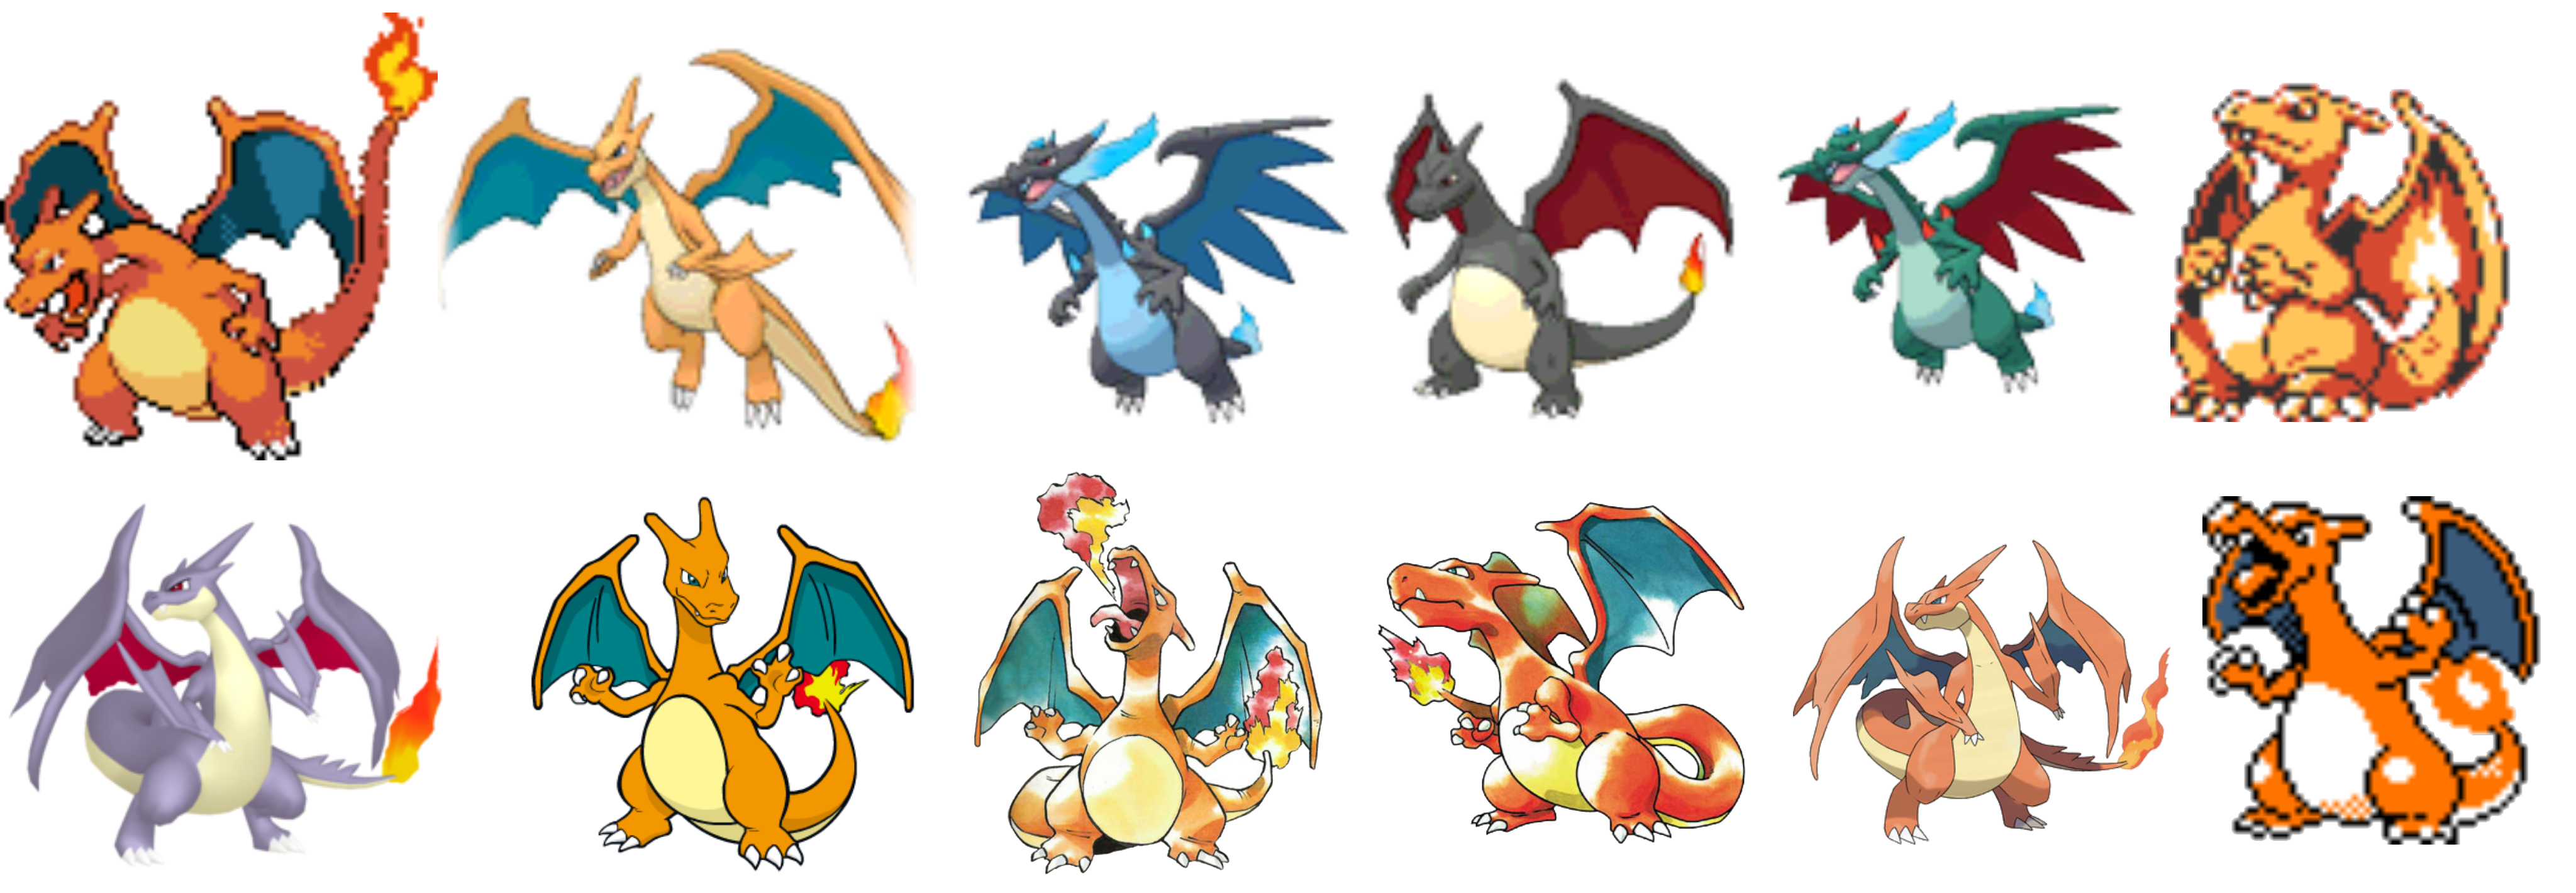
\includegraphics[width=\linewidth]{src/Images/various_charizard}
	\caption[Different Pokémon renditions]{Different renditions of the same Pokémon. Both samples from the artwork and sprite dataset are presented}
	\label{fig:variouscharizard}
\end{figure}

Note that the trained model is a conditional diffusion model, thus the samples should be categorized in a logical scheme.  There are multiple approaches on how the samples can be grouped. Typically, Pokémon are grouped based on their typing \footnote{Typing refers to the elemental or thematic category (fire, water, ghost, fairy etc.) that a Pokémon belongs to. Each Pokémon has one or two types, which determine its strengths and weaknesses in battles. There are 18 different types in total, and each type has its own set of interactions with other types.}. However, optimally similar images are grouped together. Pokémon belonging to the same type can differ drastically in regards to their appearance. Therefore, we opted to group samples based on the body from the Pokémon. 
This resulted in following classes.\\

Pokémon with: 

\begin{multicols}{3}
	\begin{enumerate}[itemsep=2pt,parsep=2pt]
		\item only a head
		\item a head and legs
		\item fins
		\item insectoid body
		\item quadruped body
		\item single pair of wings
		\item multiple bodies
		\item tentacles
		\item base and legs
		\item bipedal with tail
		\item bipedal without tail
		\item two or more pairs of wings
		\item serpentine body
		\item a head and arms
	\end{enumerate}
\end{multicols}

\begin{figure}[h]
	\centering
	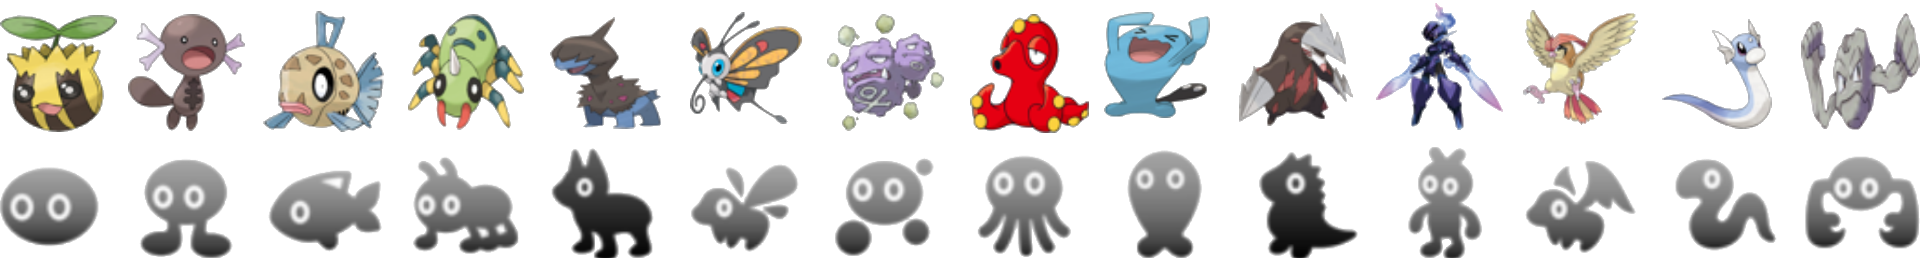
\includegraphics[width=\linewidth]{src/Images/bodyCategorys}
	\caption[Body Categories]{Different body types used to categorise the Pokémon.}
	\label{fig:bodycategorys}
\end{figure}

\subsection{Preprocessing}
The next problem we encountered was the difference in their background, their image mode and
type. At first we resize every image to 64x64. The original artwork and sprites were all transparent ”.png”, meaning they have no background and therefore a fourth channel encoding the transparency of the given pixel. This fourth channel resulted in partially transparent Pokémon and added unnecessary parameters to the network. Therefore we converted each of the ”RGBA”
images to uniform ”RGB” images with a white background to keep their characteristic black outlining. \\
As the alternative artworks were collected from a variety of different artists there was no convention resulting in different file types (jpg, jpeg and vector png), backgrounds and image modes.
To keep the format we established in the previous step we again removed the additional transparency channel and converted each image to png. Additionally, we detected each image which did not have a white background and adjusted it accordingly.\\
 Moreover, was there a difference
in coverage of the image. While the artworks used all available space of the image the sprites only used around 10\% therefore exposing a lot of white background. This was apparent after training a few test epochs which resulted in solely white images with a small focus somewhere in the center (which was no surprise as the sprites represented the majority of the dataset). To counteract this, we located the focus point of the image (location of Pokémon) by removing
each row/column only containing white pixels. Then to avoid morphing the shape of the Pokémon we padded it to a square. At last we again resized the cropped image to get a uniform size of 64x64 pixels.\\
The code for making the images uniform can be found \href{https://github.com/mhueppe/Diffusion_Models/blob/master/preprocessing/preprocessing_uniform_data.py}{here}.

An example for a sample before and after applying the uniform process can be seen in Figure \ref{fig:preprocessingpipeline}.

\begin{figure}[h]
	\centering
	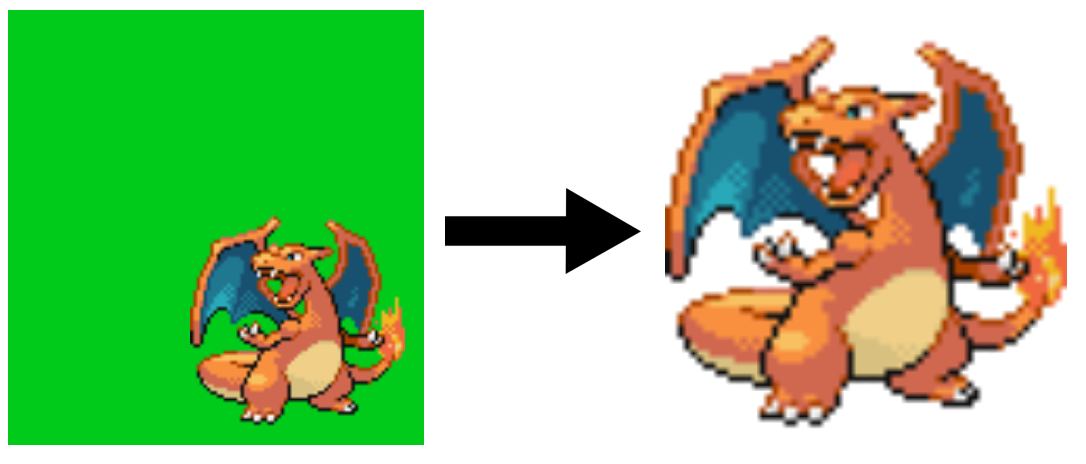
\includegraphics[width=0.5\linewidth]{src/Images/preprocessing_pipeline}
	\caption[Before and After Uniform Process]{A sample before and after applying the uniform process.}
	\label{fig:preprocessingpipeline}
\end{figure}

%
\section{Model}
\label{sec:model}
The model employed was based on the \ac{DDPM} presented by \cite{Ho2020}. \cite{Ho2020} presents both an unconditional Model and a conditional one. For generating the images we only employed the conditional architecture. However, the architecture was slightly modified. The most significant change was the implementation of a scale factor which gives the ability to increase/decrease the amount of model parameters. 

\section{Model training}
\label{sec:model_training}

\section{Results}\label{sec:results}
The following describes the results reported on both the \href{https://www.cs.toronto.edu/~kriz/cifar.html}{cifar10} dataset and our own Pokémon dataset. Since the quality of the generated image is somewhat subjective the \ac{MSE} during training is presented as well. 


\subsection{CIFAR-10}
To validate the model pipeline we first trained the model on the \href{https://www.cs.toronto.edu/~kriz/cifar.html}{cifar10} dataset since the model has already reported good results on this data. The CIFAR-10 dataset is a collection of 60,000 32x32 color images in 10 different classes, with 6,000 images per class. Each image belongs to one of the following classes:

\begin{multicols}{3}
	\begin{enumerate}[itemsep=2pt,parsep=2pt]
		\item airplane
		\item car
		\item bird
		\item cat
		\item deer
		\item dog
		\item frog 
		\item horse
		\item ship
		\item truck
	\end{enumerate}
\end{multicols}

Similarly, our model reported good results as well. 

Figure (TBA) shows the decrease of \ac{MSE} over time. 
Figure (TBA) shows the predicted images over time. As one can see the images predicted in the early stages of training were not reminiscent of the input data and mostly show either random noise or images containing only one colour. Similar to how the \ac{MSE} decreased over time the quality of the images increased. The final images clearly depict objects of the respected class. 

\section{Discussion}
\label{sec:discussion}
Our model showed good results both on the benchmark dataset and our own created dataset. The diffusion model and the increased size of the dataset showed to positively influence the quality of the predicted images. Our images had a more recognizable design than previous studies (see Figure \ref{fig:kleiberresults} \& \ref{fig:chambelresults} ). This was expected since generative models are known to work best with larger datasets \citep{Yang2023}. Additionally, \ac{DDPM}s show to generate higher quality images than simple \ac{GAN}s \citep{Guarnera2023}.

\section{Conclusion}
\label{sec:conclusion}

\begin{itemize}
	\item How are the results of this study usable? 
	\item Shortcomings of our study What was especially difficult? 	 
	\item How can the results be improved upon? 
	\item What might be further test that can be done to improve the generality? 
\end{itemize}

%%%%%%%%%%%%%%%%%%%%%%%%%%%%%%%%%%%%%%
% hier werden - zum Ende des Textes - die bibliographischen Referenzen
% eingebunden
%
% Insbesondere stehen die eigentlichen Informationen in der Datei
% ``bib.bib''
%
\printbibliography[heading=bibintoc]

\end{document}